% !TEX program = pdflatex
% 巨磁电阻效应实验报告
\documentclass[UTF8,10pt,a4paper]{article}
\usepackage{ctex}
% \catcode`\。=\active
% \newcommand{。}{.}
\newcommand{\CourseName}{近代物理实验}
\newcommand{\CourseCode}{PHYS1701}
\newcommand{\Semester}{2019-2020学年第学期}
\newcommand{\ProjectName}{巨磁电阻效应实验报告}
\newcommand{\TimeType}{实验日期}
\newcommand{\Time}{2020. 6. 10(周三)}
\newcommand{\StudentName}{陈稼霖}
\newcommand{\StudentID}{45875852}
\usepackage[vmargin=1in,hmargin=.5in]{geometry}
\usepackage{fancyhdr}
\usepackage{lastpage}
\usepackage{calc}
\pagestyle{fancy}
\fancyhf{}
\fancyhead[L]{\CourseName}
\fancyhead[C]{\ProjectName}
\fancyhead[R]{\StudentName}
\fancyfoot[R]{\thepage\ / \pageref{LastPage}}
\setlength\headheight{12pt}
\fancypagestyle{FirstPageStyle}{
    \fancyhf{}
    \fancyhead[L]{\CourseName\\
        \CourseCode\\
        \Semester}
    \fancyhead[C]{{\huge\bfseries\ProjectName}\\
        \TimeType\ : \Time}
    \fancyhead[R]{姓名 : \makebox[\widthof{\StudentID}][s]{\StudentName}\\
        学号 : \StudentID\\
        成绩 : \underline{\makebox[\widthof{\StudentID}]{}}}
    \fancyfoot[R]{\thepage\ / \pageref{LastPage}}
    \setlength\headheight{36pt}
}
\usepackage{amsmath,amssymb,amsthm,bm}
\allowdisplaybreaks[4]
\providecommand{\abs}[1]{\left\lvert#1\right\rvert}
% \usepackage{multirow}
\usepackage{graphicx}
% \usepackage{subfigure}
\begin{document}
\thispagestyle{FirstPageStyle}
\section{实验数据处理和分析}
\subsection{实验一:了解巨磁电阻效应原理,测量不同磁场下的巨磁电阻阻值$R_B$,做$R_B/R_0-B$关系图,求电阻相对变化率$(R_B-R_0)/R_0$的最大值}

将白色波段开关拨至B点,此时等效实验电路如图\ref{circuit-1}.

\begin{figure}[h]
    \centering
    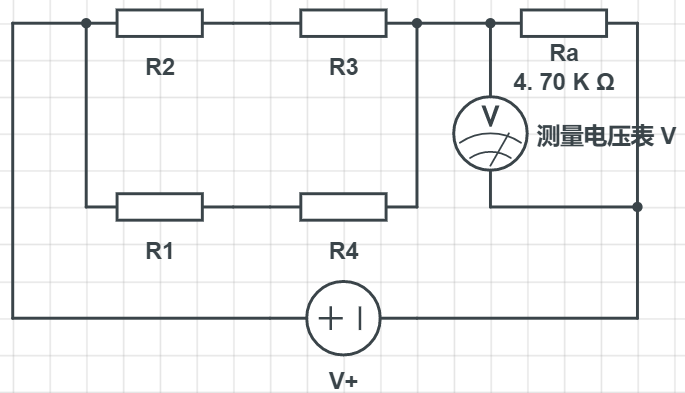
\includegraphics[width=.4\textwidth]{Circuit-1.png}
    \caption{实验一等效电路图}
    \label{circuit-1}
\end{figure}

设定传感器工作电压$V_+=3.003$V,在线圈电流$I=0$时,即无磁场时的测量电压表输出为$V_0=1.5168$V,因此左边四个并联的电阻等效而成的阻值(即一个巨磁电阻在无磁场情况下的阻值)为
\begin{align}
    R_0=\frac{V_+-V_0}{V_0}R_a=\frac{3.003-1.5168}{1.5168}\times 4.70\times 10^3\Omega=4.61\times 10^{3}\Omega,
\end{align}
以$0.05$A为步长从$0$开始逐渐升高线圈电流,即增大施加在巨磁电阻上的磁场,此时巨磁电阻的阻值逐渐减小,从而左边这个并联电路的阻值逐渐减小,$R_a$分到的电压逐渐增大,即测量电压表的输出逐渐增大,我们记录了测量电压表输出值$V$随着线圈电流$I$变化的数据,见表\ref{1-T}第1和3列.

左边并联电路中的四个巨磁电阻完全相同,在未施加磁场的情况下$R_1=R_2=R_3=R_4=R_0$. 但只有$R_1$和$R_3$两个电阻受磁场影响而改变阻值,当施加磁场,$R_1=R_3=R_B$;由于在磁性材料的下方被屏蔽而不受磁场影响,电阻不变,$R_2=R_4=R_0$. 并联电路中的四个电阻等效为一只巨磁电阻,当未施加磁场时,其阻值为
\begin{align}
    R_X=R_0,
\end{align}
当施加磁场时,其阻值为
\begin{align}
    \label{RX}
    R_X=\frac{1}{2}(R_B+R_0).
\end{align}
同时,由并联的四个电阻和$R_a$之间的分压,又有
\begin{align}
    \label{RX2}
    R_X=\frac{V_+-V}{V}R_a.
\end{align}
利用式\eqref{RX}和式\eqref{RX2}有
\begin{align}
    R_B=2\frac{V_+-V}{V}R_a-R_0,
\end{align}
从而可以利用表\ref{1-T}第2列的测量电压表输出电压$V$计算出磁场下单个巨磁电阻阻值$R_B$,见表\ref{1-T}第4列,计算磁场下阻值与无磁场阻值之比$R_B/R_0$见表\ref{1-T}第5列,电阻相对变化率$(R_B-R_0)/R_0$见表\ref{1-T}第6列.

我们向巨磁电阻施加磁场所使用的线圈是亥姆霍兹线圈,巨磁电阻被置于亥姆霍兹线圈的中央. 亥姆霍兹线圈是一对同轴等大的圆形线圈,两个线圈的间距等于线圈的半径. 根据Biot-Savart定律,亥姆霍兹线圈在其中央产生的磁感应强度为
\begin{align}
    \label{B}
    B=2\times\frac{\mu_0nIR^2}{2(R^2+(R/2)^2)^{3/2}}=\left(\frac{4}{5}\right)^{3/2}\frac{\mu_0nI}{R}
\end{align}
其中线圈匝数$N=200$,半径$R=0.100$m. 利用上式计算亥姆霍兹线圈施加在巨磁电阻上的磁感应强度,见表\ref{1-T}第2列.

\begin{table}[h]
    \scriptsize
    \centering
    \caption{实验一数据记录表}
    \label{1-T}
    \begin{tabular}{|c|c|c|c|c|c|}
    \hline
    \begin{tabular}[c]{@{}c@{}}线圈电流\\ $I$ / A\end{tabular} & \begin{tabular}[c]{@{}c@{}}亥姆霍兹线圈施加在\\ 巨磁电阻上的\\ 磁感应强度 $B$ / T\end{tabular} & \begin{tabular}[c]{@{}c@{}}电压表示数\\ $V$ / V\end{tabular} & \begin{tabular}[c]{@{}c@{}}磁场下\\ 单个巨磁电阻的\\ 阻值 $R_B$ / $\Omega$\end{tabular} & \begin{tabular}[c]{@{}c@{}}磁场下巨磁电阻阻值\\ 和无磁场阻值的\\ 比值 $R_B/R_0$\end{tabular} & \begin{tabular}[c]{@{}c@{}}巨磁电阻阻值相对变化率\\ $(R_B-R_0)/R_0$\end{tabular} \\ \hline
    0.000 & 0E+00 & 1.5168 & 4.61E+03 & 1.00 & 0.00 \\ \hline
    0.050 & 9.0E-05 & 1.5185 & 4.6E+03 & 1.0 & -0.0045 \\ \hline
    0.100 & 1.80E-04 & 1.5202 & 4.56E+03 & 0.991 & -0.00904 \\ \hline
    0.150 & 2.70E-04 & 1.5222 & 4.54E+03 & 0.986 & -0.0143 \\ \hline
    0.200 & 3.60E-04 & 1.5246 & 4.51E+03 & 0.979 & -0.0207 \\ \hline
    0.250 & 4.50E-04 & 1.5267 & 4.48E+03 & 0.974 & -0.0262 \\ \hline
    0.300 & 5.40E-04 & 1.5290 & 4.46E+03 & 0.968 & -0.0322 \\ \hline
    0.350 & 6.29E-04 & 1.5314 & 4.43E+03 & 0.961 & -0.0385 \\ \hline
    0.400 & 7.19E-04 & 1.5339 & 4.40E+03 & 0.955 & -0.0451 \\ \hline
    0.450 & 8.09E-04 & 1.5363 & 4.37E+03 & 0.949 & -0.0513 \\ \hline
    0.500 & 8.99E-04 & 1.5390 & 4.34E+03 & 0.942 & -0.0583 \\ \hline
    0.550 & 9.89E-04 & 1.5416 & 4.31E+03 & 0.935 & -0.0650 \\ \hline
    0.600 & 1.08E-03 & 1.5440 & 4.28E+03 & 0.929 & -0.0712 \\ \hline
    0.650 & 1.17E-03 & 1.5467 & 4.25E+03 & 0.922 & -0.0781 \\ \hline
    0.700 & 1.26E-03 & 1.5492 & 4.22E+03 & 0.915 & -0.0845 \\ \hline
    0.750 & 1.35E-03 & 1.5516 & 4.19E+03 & 0.909 & -0.0906 \\ \hline
    0.800 & 1.44E-03 & 1.5544 & 4.16E+03 & 0.902 & -0.0978 \\ \hline
    0.850 & 1.53E-03 & 1.5563 & 4.13E+03 & 0.897 & -0.103 \\ \hline
    0.900 & 1.62E-03 & 1.5581 & 4.11E+03 & 0.893 & -0.107 \\ \hline
    0.950 & 1.71E-03 & 1.5596 & 4.09E+03 & 0.889 & -0.111 \\ \hline
    1.000 & 1.798E-03 & 1.5607 & 4.08E+03 & 0.886 & -0.114 \\ \hline
    1.050 & 1.888E-03 & 1.5613 & 4.07E+03 & 0.885 & -0.115 \\ \hline
    1.100 & 1.978E-03 & 1.5617 & 4.07E+03 & 0.884 & -0.116 \\ \hline
    1.150 & 2.068E-03 & 1.5619 & 4.07E+03 & 0.883 & -0.117 \\ \hline
    1.200 & 2.158E-03 & 1.5620 & 4.07E+03 & 0.883 & -0.117 \\ \hline
    1.250 & 2.248E-03 & 1.5620 & 4.07E+03 & 0.883 & -0.117 \\ \hline
    1.300 & 2.338E-03 & 1.5621 & 4.07E+03 & 0.883 & -0.117 \\ \hline
    1.350 & 2.428E-03 & 1.5621 & 4.07E+03 & 0.883 & -0.117 \\ \hline
    1.400 & 2.518E-03 & 1.5622 & 4.06E+03 & 0.883 & -0.117 \\ \hline
    1.450 & 2.608E-03 & 1.5622 & 4.06E+03 & 0.883 & -0.117 \\ \hline
    1.500 & 2.698E-03 & 1.5622 & 4.06E+03 & 0.883 & -0.117 \\ \hline
    \end{tabular}
    \normalsize
\end{table}

绘制$R_B/R_0-B$关系图如图\ref{1-F}.

\begin{figure}[h]
    \centering
    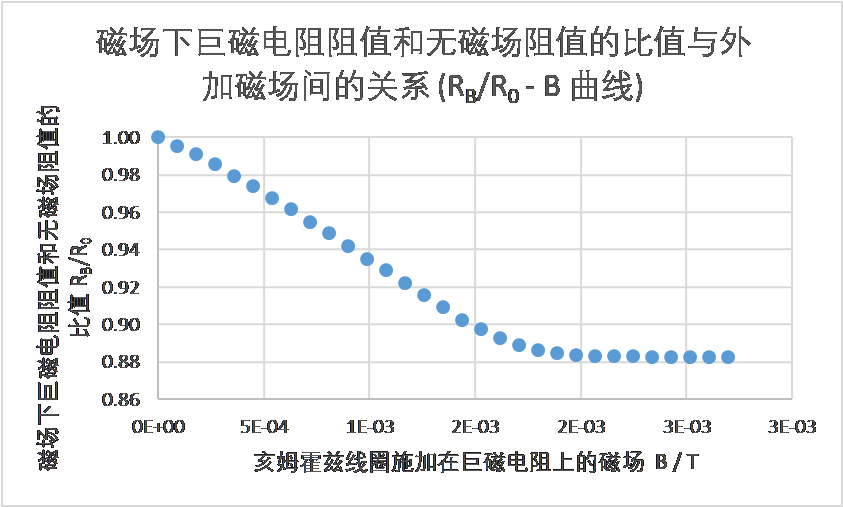
\includegraphics[width=.6\textwidth]{1-F.png}
    \caption{磁场下巨磁电阻阻值和无磁场阻值的比值与外加磁感应强度间的关系 ($R_B/R_0 - B$ 曲线)}
    \label{1-F}
\end{figure}

电阻相对变化率的绝对值$\abs{(R_B-R_0)/R_0}$的最大值为$11.7\%$.

\clearpage

\subsection{实验二:学习据此电阻传感器定标方法,计算巨磁电阻传感器灵敏度,由巨磁电阻传感器输出电压$V_{\text{输出}}$,得到电阻相对变化率$(R_B-R_0)/R_0$的最大值}

将传感器输出表头下的放大倍数档调至$\times 1$档,将测量电压表下的白色波段开关拨向A点,此时等效实验电路如图\ref{circuit-2}.

\begin{figure}[h]
    \centering
    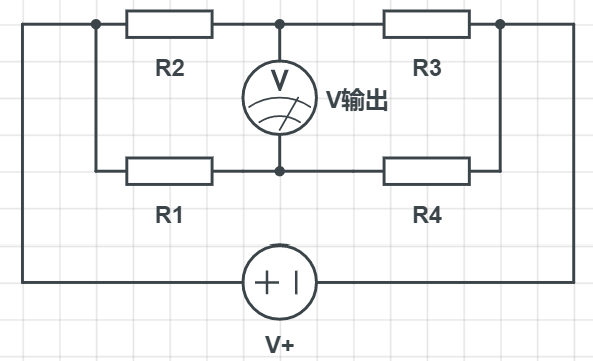
\includegraphics[width=.4\textwidth]{Circuit-2.png}
    \caption{实验二/三等效电路图}
    \label{circuit-2}
\end{figure}

设定传感器工作电压$V_+=4.992$V,线圈电流为$0$,将传感器输出电压调零. 以$0.05$A为步长从$0$开始逐渐升高线圈电流,即增大施加在巨磁电阻上的磁场,$R_1$和$R_3$阻值减小,电桥中电压表两端的电势差增大,巨磁电阻传感器(即电桥中的电压表)输出增大,我们记录了巨磁电阻传感器输出电压$V_{\text{输出}}$随着线圈电流$I$变化的数据,见表\ref{2-T}第1和3列. 用式\ref{B},计算各个线圈$I$对应的亥姆霍兹线圈施加在巨磁电阻上的磁感应强度,如表\ref{2-T}第2列.

惠斯通电桥的输出电压为
\begin{align}
    \label{Vout}
    V_{\text{输出}}=V_+\frac{R_0-R_B}{R_0+R_B}
\end{align}
故
\begin{align}
    \frac{R_B-R_0}{R_0}=-2\frac{V_{\text{输出}}}{V_++V_{\text{输出}}},
\end{align}
利用上式计算各个磁感应强度下,巨磁电阻阻值的相对变化率,见表\ref{2-T}第4列,得到巨磁电阻阻值相对变化率绝对值的最大值
\[
    \abs{(R_B-R_0)/R_0}_{\max}=11.7\%,
\]
与实验一得到的数值一致.

\begin{table}[h]
    \footnotesize
    \centering
    \caption{实验二数据记录表}
    \label{2-T}
    \begin{tabular}{|c|c|c|c|}
        \hline
        \begin{tabular}[c]{@{}c@{}}线圈电流\\ $I$ / A\end{tabular} & \begin{tabular}[c]{@{}c@{}}亥姆霍兹线圈施加在巨磁电阻上的\\ 磁感应强度 $B$ / T\end{tabular} & \begin{tabular}[c]{@{}c@{}}巨磁电阻传感器\\ 输出电压 $V_{\text{输出}}$ / V\end{tabular} & \begin{tabular}[c]{@{}c@{}}巨磁电阻阻值\\ 相对变化率 $(R_B-R_0)/R_0$\end{tabular} \\ \hline
        0.000 & 0E+00 & 0.000 & 0.000 \\ \hline
        0.050 & 9.0E-05 & 0.010 & -0.004 \\ \hline
        0.100 & 1.80E-04 & 0.021 & -0.008 \\ \hline
        0.150 & 2.70E-04 & 0.034 & -0.014 \\ \hline
        0.200 & 3.60E-04 & 0.048 & -0.019 \\ \hline
        0.250 & 4.50E-04 & 0.063 & -0.025 \\ \hline
        0.300 & 5.40E-04 & 0.080 & -0.032 \\ \hline
        0.350 & 6.29E-04 & 0.096 & -0.038 \\ \hline
        0.400 & 7.19E-04 & 0.113 & -0.044 \\ \hline
        0.450 & 8.09E-04 & 0.130 & -0.051 \\ \hline
        0.500 & 8.99E-04 & 0.148 & -0.058 \\ \hline
        0.550 & 9.89E-04 & 0.165 & -0.064 \\ \hline
        0.600 & 1.08E-03 & 0.185 & -0.071 \\ \hline
        0.650 & 1.17E-03 & 0.200 & -0.077 \\ \hline
        0.700 & 1.26E-03 & 0.218 & -0.084 \\ \hline
        0.750 & 1.35E-03 & 0.235 & -0.090 \\ \hline
        0.800 & 1.44E-03 & 0.252 & -0.096 \\ \hline
        0.850 & 1.53E-03 & 0.268 & -0.102 \\ \hline
        0.900 & 1.62E-03 & 0.281 & -0.107 \\ \hline
        0.950 & 1.71E-03 & 0.292 & -0.111 \\ \hline
        1.000 & 1.798E-03 & 0.299 & -0.113 \\ \hline
        1.050 & 1.888E-03 & 0.303 & -0.114 \\ \hline
        1.100 & 1.978E-03 & 0.306 & -0.116 \\ \hline
        1.150 & 2.068E-03 & 0.307 & -0.116 \\ \hline
        1.200 & 2.158E-03 & 0.307 & -0.116 \\ \hline
        1.250 & 2.248E-03 & 0.308 & -0.116 \\ \hline
        1.300 & 2.338E-03 & 0.308 & -0.116 \\ \hline
        1.350 & 2.428E-03 & 0.308 & -0.116 \\ \hline
        1.400 & 2.518E-03 & 0.309 & -0.117 \\ \hline
        1.450 & 2.608E-03 & 0.309 & -0.117 \\ \hline
        1.500 & 2.698E-03 & 0.309 & -0.117 \\ \hline
    \end{tabular}
    \normalsize
\end{table}

以传感器输出电压$V_{\text{输出}}$为纵轴,以亥姆霍兹施加在巨磁电阻上的磁感应强度$B$为横轴,做图\ref{2-F}. 由图\ref{2-F}可见,巨磁电阻传感器输出电压先随着磁场的增大而近似于线性增大,当磁感应强度$B>2.00\times 10^{-3}$T之后,传感器的输出电压不再随着磁场的增加有显著变化. 我们将巨磁电阻传感器的灵敏度定义为传感器输出电压关于磁感应强度在线性递增范围内的斜率,对于$B<2.00\times 10^{-3}$T范围内的数据点进行拟合(由于在测量前已经将输出电压调零,故拟合线应当准确地经过零点),得到巨磁电阻传感器的灵敏度为$167$V/T.

\begin{figure}[h]
    \centering
    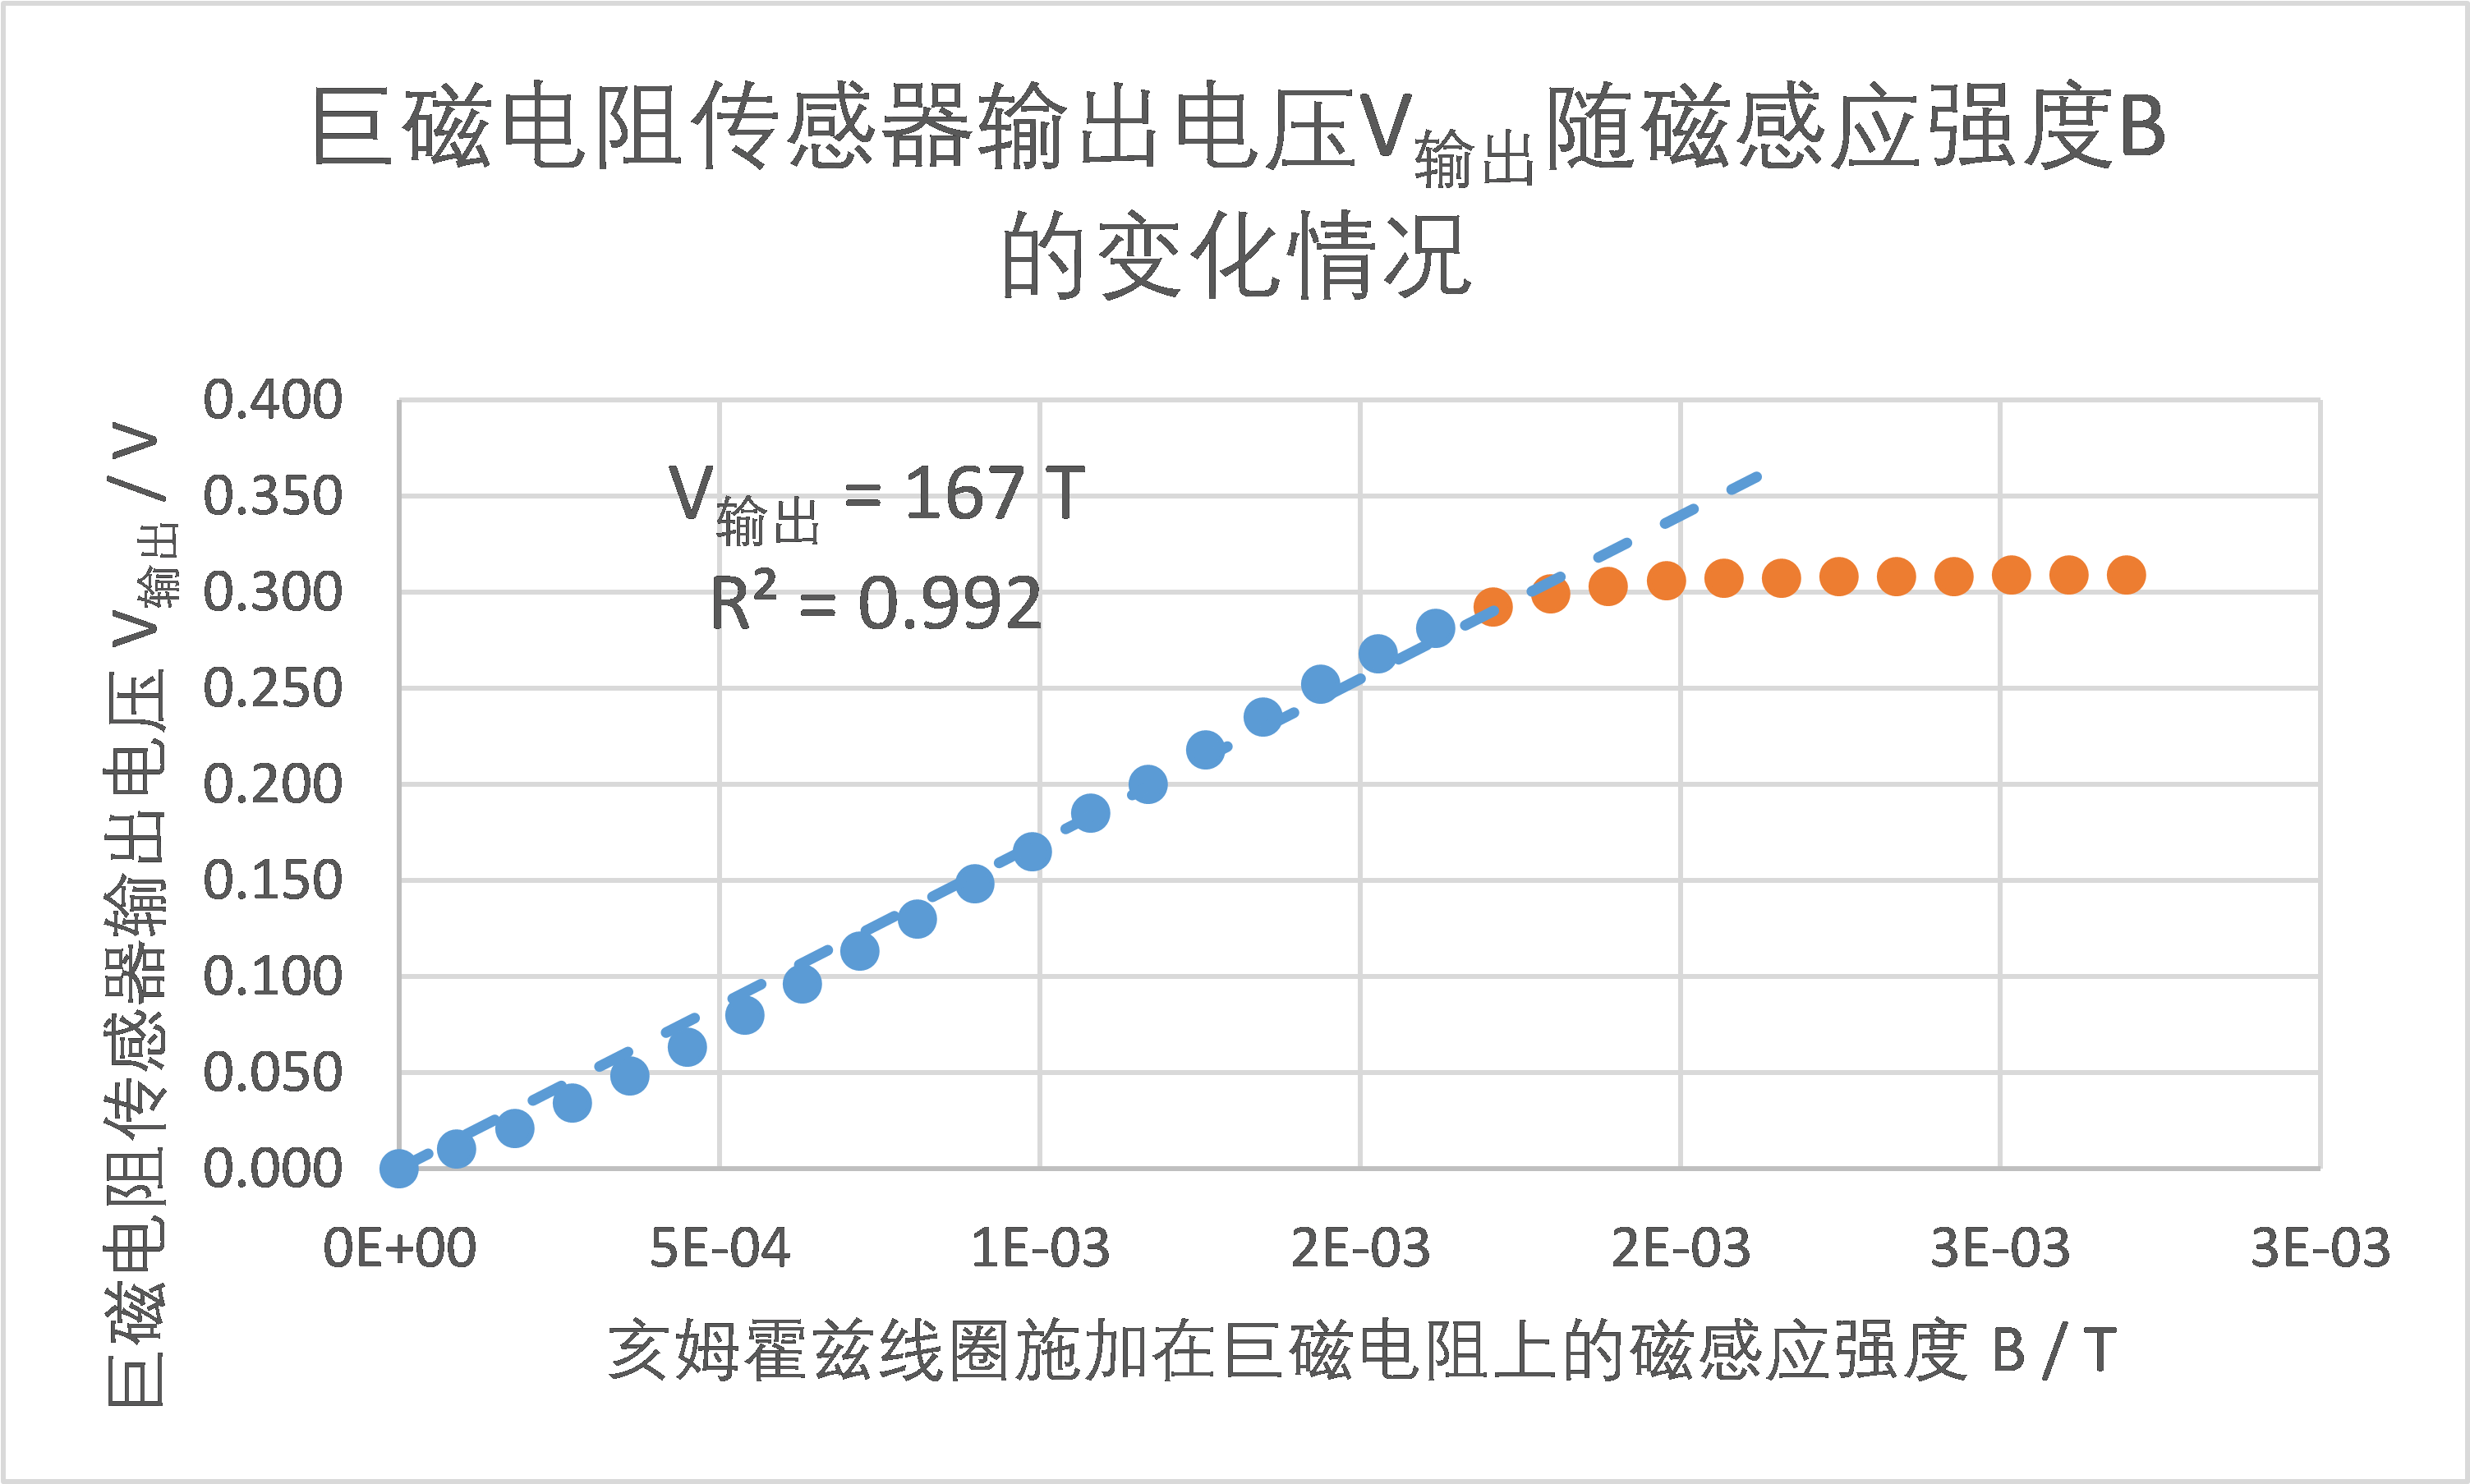
\includegraphics[width=.6\textwidth]{2-F.png}
    \caption{巨磁电阻传感器输出电压$V_{\text{输出}}$随磁感应强度$B$的变化情况}
    \label{2-F}
\end{figure}

\clearpage

\subsection{实验三:测定巨磁电阻传感器输出电压$V_{\text{输出}}$与其工作电压$V_+$的关系}

将传感器输出表头下的放大倍数档调至$\times 1$档,将测量电压表下的白色波段开关拨向A点,此时等效实验电路仍如图\ref{circuit-2}. 设定传感器工作电压$V_+=2.000$V,将传感器输出电压调零,设定线圈电流$I=0.600$A,以大约$1.000$V为步长从$0$开始逐渐增大传感器工作电压,我们记录了传感器输出电压$V_{\text{输出}}$随传感器工作电压增大的数据,见表\ref{3-T}.

\begin{table}[h]
    \centering
    \caption{实验三数据记录表}
    \label{3-T}
    \begin{tabular}{|c|c|}
    \hline
    \begin{tabular}[c]{@{}c@{}}巨磁电阻传感器工作电压\\ $V_+$ / V\end{tabular} & \begin{tabular}[c]{@{}c@{}}巨磁电阻传感器输出电压\\ $V_{\text{输出}}$ / V\end{tabular} \\ \hline
    2.000 & 0.073 \\ \hline
    2.999 & 0.113 \\ \hline
    4.002 & 0.153 \\ \hline
    5.003 & 0.193 \\ \hline
    5.999 & 0.233 \\ \hline
    7.003 & 0.273 \\ \hline
    8.004 & 0.313 \\ \hline
    8.998 & 0.353 \\ \hline
    10.000 & 0.393 \\ \hline
    11.003 & 0.433 \\ \hline
    12.000 & 0.472 \\ \hline
    12.998 & 0.512 \\ \hline
    \end{tabular}
\end{table}

由式\eqref{Vout}知传感器输出电压$V_{\text{输出}}$与传感器工作电压之间呈线性关系,斜率为$\frac{R_0-R_B}{R_0+R_B}$. 以传感器输出电压$V_{\text{输出}}$为纵轴,以其工作电压$V_+$为横轴做图\ref{3-F},线性拟合得到斜率
\[
    \frac{(R_0-R_B)}{(R_0+R_B)}=0.0399.
\]
从这一斜率中还可以倒推出此时巨磁电阻的阻值为
\[
    R_B=4.25\times 10^3\Omega,
\]
这一数值与实验一中得到的电流$I=0.600$A对应的巨磁电阻阻值$R_B=4.28\times 10^3\Omega$相符合.

\begin{figure}[h]
    \centering
    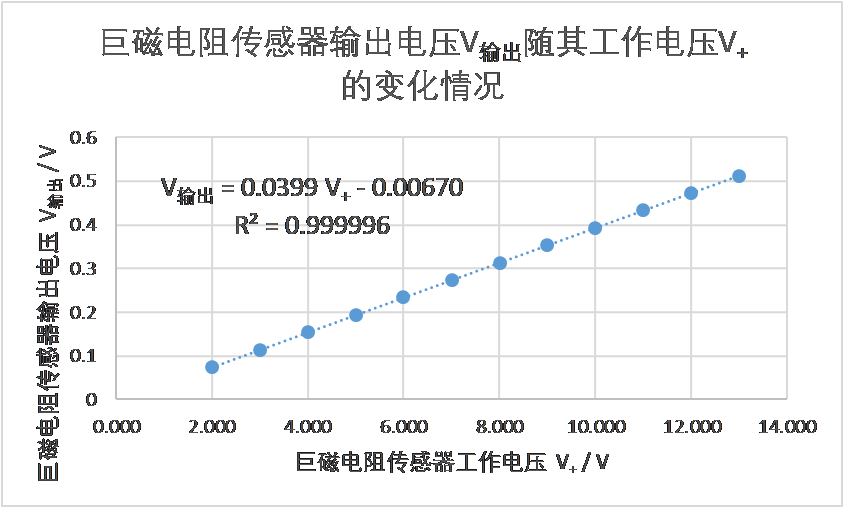
\includegraphics[width=.5\textwidth]{3-F.png}
    \caption{巨磁电阻传感器输出电压$V_{\text{输出}}$随其工作电压$V_+$的变化情况}
    \label{3-F}
\end{figure}

\clearpage

\subsection{实验四:测定巨磁电阻传感器输出电压$V_{\text{输出}}$与通电导线电流$I$的关系}

将传感器输出表头下的放大倍数档调至$\times 10$档,将测量电压表下的白色波段开关拨向A点. 设定传感器工作电压$V_+=5.000$V,巨磁电阻传感器输出调零,以$0.50$A为步长从$0$逐渐升高被测电流,此时施加在巨磁电阻上的磁场逐渐增大,巨磁电阻的阻值逐渐减小,传感器输出逐渐增大,我们记录了传感器输出电压$V_{\text{输出}}$随待测电流变化的数据,见表\ref{4-T}.

\begin{table}[h]
    \centering
    \caption{实验四数据记录表}
    \label{4-T}
    \begin{tabular}{|c|c|}
    \hline
    \begin{tabular}[c]{@{}c@{}}待测电流\\ $I$ / A\end{tabular} & \begin{tabular}[c]{@{}c@{}}传感器输出电压\\ $V_{\text{输出}}$ / V\end{tabular} \\ \hline
    0.50 & 0.015 \\ \hline
    1.00 & 0.028 \\ \hline
    1.50 & 0.043 \\ \hline
    2.00 & 0.057 \\ \hline
    2.50 & 0.068 \\ \hline
    3.00 & 0.085 \\ \hline
    3.50 & 0.100 \\ \hline
    4.00 & 0.114 \\ \hline
    4.50 & 0.128 \\ \hline
    5.00 & 0.144 \\ \hline
    5.41 & 0.157 \\ \hline
    \end{tabular}
\end{table}

由实验二知,在一定范围内,巨磁电阻传感器的输出电压$V_{\text{输出}}$正比于磁感应强度$B$
\begin{align}
    V_{\text{输出}}=KB,
\end{align}
而根据Search Results定理,无限长直导线在距其$d$处产生的磁感应强度为
\begin{align}
    B=\frac{\mu_0I}{2\pi d},
\end{align}
故传感器输出电压$V_{\text{输出}}$应当与待测电流成正比
\begin{align}
    V_{\text{输出}}=K\frac{\mu_0I}{2\pi d}.
\end{align}
以传感器输出电压$V_{\text{输出}}$为纵轴,以待测电流$I$为横轴做图\ref{4-F},线性拟合发现数据点的线性性质果然非常好,可见实验和理论相符,线性拟合得到的斜率为$0.0286$V/A.

\begin{figure}[h]
    \centering
    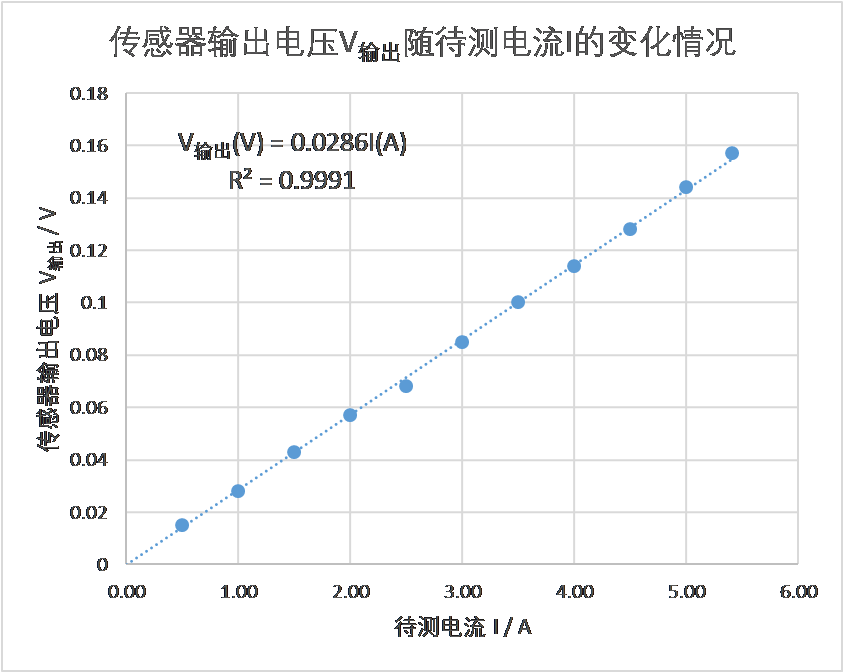
\includegraphics[width=.6\textwidth]{4-F.png}
    \caption{传感器输出电压$V_{\text{输出}}$随待测电流$I$的变化情况}
    \label{4-F}
\end{figure}

理论上,我们可以根据图\ref{4-F}的斜率推算出待测电流所在的导线与巨磁电阻的距离:
\begin{align}
    K\frac{\mu_0}{2\pi d}\times 10=0.0286\text{V}/\text{A},\quad\Longrightarrow d=1.17\times 10^{-2}\text{m}=1.17\text{cm}.
\end{align}
(注意我们这里乘了$10$,这是因为本实验中我们的传感器输出放大倍数为$\times 10$.)\\
但是考虑到待测电流所在的导线与巨磁电阻的距离和巨磁电阻本身的尺寸大小相当,因此待测电流在巨磁电阻上形成的磁场可能并不很均匀,如此计算得到的距离可能并不是很准确,仅做参考.

\clearpage

\subsection{拓展实验:地磁场的测量}

前面的实验中要求注意地磁场对实验产生的影响,因此我们在实验过程中始终保持仪器位置、朝向不变,这样可以保证巨磁电阻感受到的地磁场不变,从而避免影响实验. 现在我们来测量一下地磁场的大小,看看它究竟能在多大量级上影响我们的传感器输出.

\textbf{实验步骤}:
\begin{enumerate}
    \item 按照实验二的电路连接各器材(将测量电压表下的白色波段开关拨向$A$点),将传感器输出表头下的放大倍数调至$\times 1$档,设定传感器工作电压$V_+=5.000$V,线圈电流和被测电流都设为$0$;
    \item 考虑到实验室显然不是处于赤道上,因此当地的地磁场肯定与水平桌面存在一定夹角. 因此我们先将实验装置架平放在桌面上转动,直至传感器输出电压达到极大值,然后将实验装置架在由桌面法线和亥姆霍兹线圈轴线确定的竖直平面内转动,直至传感器输出电压达到最大值,此时,地磁场正好平行于亥姆霍兹线圈的轴线而施加在巨磁电阻上,传感器的输出电压恰好对应着正向施加的地磁场;
    \item 用与第2步同样的方法,找到传感器输出电压在地磁场下的最小值.
\end{enumerate}

\textbf{数据处理和分析}:\\
我们测得传感器输出电压的最大值为$0.029$V,最小值为$-0.040$V,这两个值之差即对应了地磁感应强度的两倍,计算得地磁场的磁感应强度为
\begin{align}
    B_{\text{地}}=\frac{(0.029+0.040)/10}{2K}\text{T}=2.1\times 10^{-5}\text{T}.
\end{align}
(这里除以$10$是因为此时传感器输出放大倍数为$\times 10$)\\
查阅资料知,地磁场的参考值在$2.5\times 10^{-5}\sim 6.5\times 10^{-5}$T范围内,可见我们的测量还是较为准确的. 我们也看到,实际上,地磁场的强度($\sim 10^{-5}T$)是远远小于我们亥姆霍兹线圈产生的磁场的($\sim 10^{-4}\sim 10^{-3}$T),因此对实验的影响还是比较有限的.

\end{document}